\section{Case Study 2: Sugarscape (Second Encounter)}
\label{sec:cs_sugarscape}

One of the first  Agent-Based Simulation model which rose to some prominence was the Sugarscape model developed by Epstein and Axtell in 1996 \cite{epstein_growing_1996}. Their aim was to \textit{grow} an artificial society by simulation and connect observations in their simulation to phenomenon of real-world societies. In this simulation a population of agents move around in a discrete 2d environment and interact with each other and the environment in many different ways. The main features of this model are (amongst others)are: searching, harvesting and consuming of resources, wealth and age distributions, population dynamics under sexual reproduction, cultural processes and transmission, combat and assimilation, bilateral decentralized trading (bartering) between agents with endogenous demand and supply, disease processes transmission and immunology.

We implemented the \textit{Carrying Capacity} (p. 30) section of Chapter II of the book \cite{epstein_growing_1996}. There, in each step agents search (move) to the cell with the most sugar they see with their vision, harvest all of it from the environment and consume sugar because of their metabolism. Sugar regrows in the environment over time. Only one agent can occupy a cell at a time. Agents don't age and cannot die from age. If agents run out of sugar due to their metabolism, they die from starvation and are removed from the simulation. In this section the authors report that the initial number of agents quickly drops and stabilises around a level depending on the model parameters. This is in accordance with our results as we show in Figure \ref{fig:vis_sugarscape} and guarantees that we don't run out of agents. The model parameters are as follows:

\begin{itemize}
	\item Sugar Endowment: each agent has an initial sugar endowment random uniform distributed between 5 and 25 units.
	\item Sugar Metabolism: each agent has a sugar metabolism random uniform distributed between 1 and 5.
	\item Agent Vision: each agent has a vision random uniform distributed between 1 and 6 in each of the 4 directions (N, W, S, E). 
	\item Sugar Growback: sugar grows back by 1.0 unit per step until the maximum capacity of a cell is reached.
	\item Agent Number: initially 500 agents.
	\item Environment Size: 50 x 50 cells with toroid boundaries which wrap around in both x and y dimension.
\end{itemize}

The model specification requires to shuffle agents before every step (Footnote 12 on page 26). In the Sequential approach we do this explicitly but in the STM approach this happens automatically due to race-conditions in concurrency thus we arrive at an effectively shuffled processing of agents: we can assume that the order of the agents is \textit{effectively} random in every step. The important difference between the two approaches is that in the State approach we have full control over this randomness but in the STM not - also this means that repeated runs with the same initial conditions might lead to slightly different results.

\begin{figure}
\begin{center}
	\begin{tabular}{c c}
		\begin{subfigure}[b]{0.4\textwidth}
			\centering
			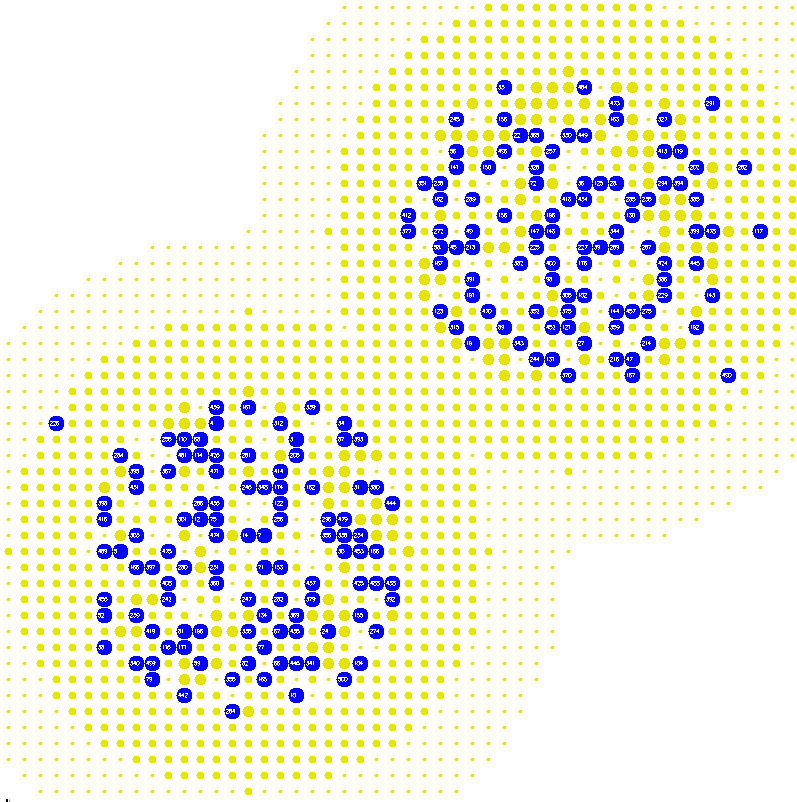
\includegraphics[width=1\textwidth, angle=0]{./fig/sugarscape/vis/sugarscape_t60_environment.png}
			\caption{Visualisation of the Sugarscape at $t = 50$.}
			\label{fig:vis_sugarscape_t50_environment}
		\end{subfigure}
    	
    	&
  
		\begin{subfigure}[b]{0.5\textwidth}
			\centering
			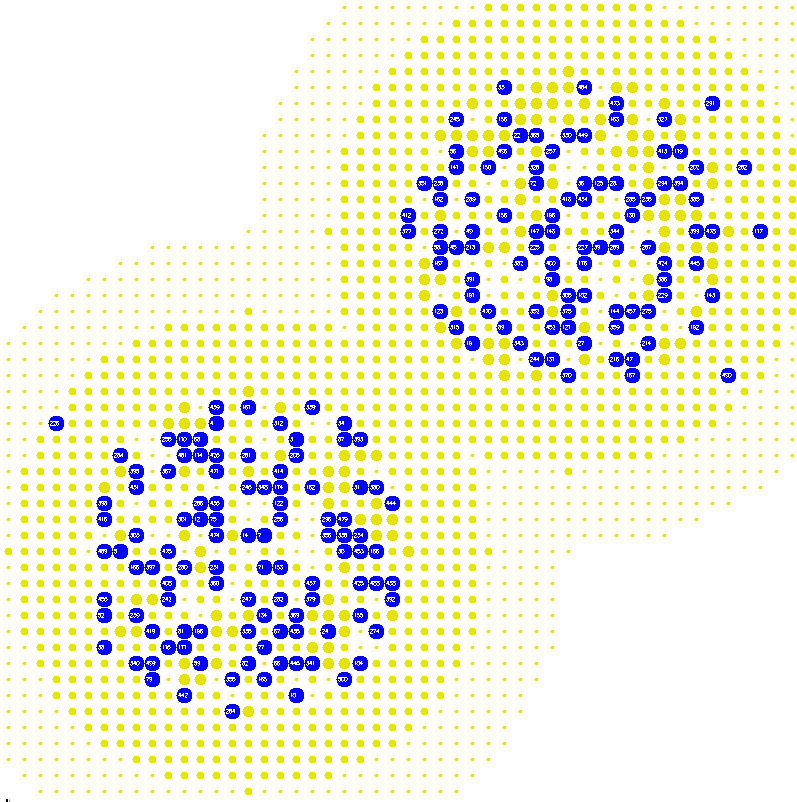
\includegraphics[width=1\textwidth, angle=0]{./fig/sugarscape/vis/sugarscape_t60_dynamics.png}
			\caption{Dynamics population size over 50 steps.}
			\label{fig:vis_sugarscape_t50_dynamics}
		\end{subfigure}
	\end{tabular}
	
	\caption{Visualisation of our SugarScape implementation and dynamics of the population size over 50 steps.}
	\label{fig:vis_sugarscape}
\end{center}
\end{figure}

\subsection{Experiment Design}
We follow \cite{lysenko_framework_2008} and measure the average updates per second of the simulation over 60 seconds.

For each experiment we conducted 8 runs on our machine (see Table \ref{tab:machine_specs}) under no additional work-load and report the average. In the experiments we varied the number of cores when running concurrently - the numbers are always indicated clearly. For varying the number of cores we compiled the executable using \textit{stack} and the \textit{threaded} option and executed it with \textit{stack} using the \textit{+RTS -Nx} option where x is the number of cores between 1 and 4. TODO main measure: steps/sec and retry-ratio

Note that we omit the graphical rendering in the functional approach because it is a serious bottleneck taking up substantial amount of the simulation time. Although visual output is crucial in ABS, it is not what we are interested here thus we completely omit it and only output the number of agents in the simulation at each step piped into a file, thus omitting slow output to the console. Note that we need to produce \textit{some} output because of Haskells laziness - if we wouldn't output anything from the simulation then the expressions would actually never be fully evaluated thus resulting in ridiculous high number of steps per second but which obviously don't really reflect the true computations done.

Note that in contrast to the SIR case-study we don't provide an IO implementation because we focus on different thing here. The focus here is on how different data-structures can make a huge impact on the performance.

\subsection{Naive Approach}
In this first approach we compare the non-concurrent \textit{Sequential} approach against an implementation using \textit{STM} where we vary the number of cores. In the \textit{STM} implementation we share the environment in the same way as in the SIR case study of Section \ref{sec:cs_sir} using a \textit{TVar}. For running the environment we implemented followed two approaches: running it asynchronously as a concurrent agent at the same time with the population agents and synchronously after all agents have run. The results are reported in Table \ref{tab:naive_results_time} and can be seen in Figure \ref{fig:naive_results_time}. 

\begin{table}
	\centering
  	\begin{tabular}{ c || c | c | c || c | c }
                   & Cores & Steps (async) & Retries (async) & Steps (sync) & Retries (sync) \\ \hline \hline 
    	Sequential & 1     & N/A           & N/A 			 & 28.2         & N/A            \\ \hline \hline    
   		STM        & 1     & 30.9          & 0.004 			 & 31.1 	    & 0.004          \\ \hline
   		STM        & 2     & 35.5          & 1.0 		     & 35.4         & 1.1 			 \\ \hline
   		STM        & 3     & 38.5          & 2.2 			 & 38.8 	    & 2.1 			 \\ \hline
   		STM        & 4     & 37.3          & 3.4             & 37.4         & 3.4
   	\end{tabular}
  	
  	\caption{Steps per second and retries on 50x50 grid and 500 initial agents using the \textit{Sequential} and \textit{TVar} on an asynchronous and synchronous environment.}
	\label{tab:naive_results_time}
\end{table}

\begin{figure}
	\centering
	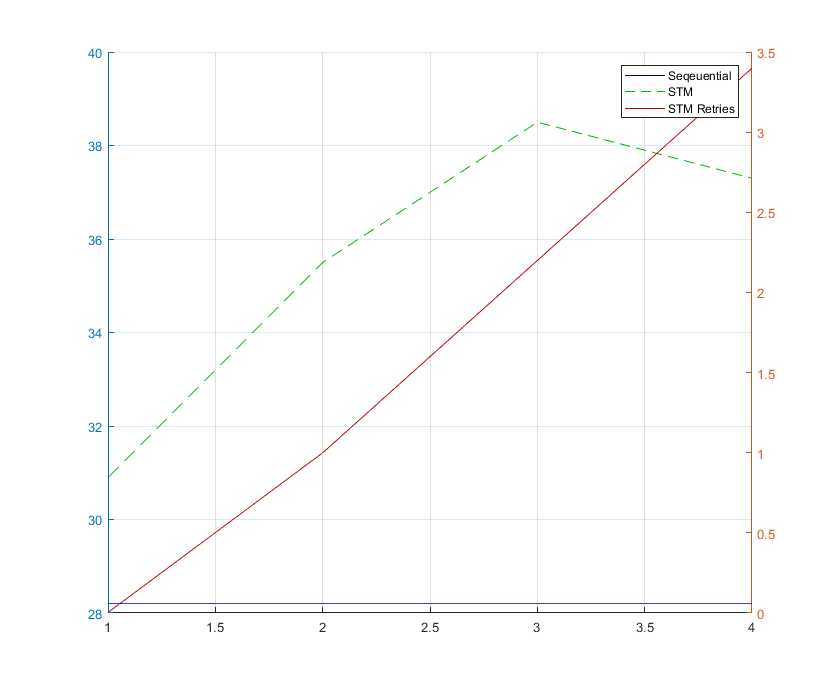
\includegraphics[width=0.6\textwidth, angle=0]{./fig/sugarscape/tvar_concenv_500_50x50.png}
	\caption{Steps per second and retries on 50x50 grid and 500 initial agents using the \textit{Sequential} and \textit{TVar} on an asynchronous and synchronous environment.}
	\label{fig:naive_results_time}
\end{figure}

Clearly the concurrent \textit{STM} implementation outperforms the \textit{Sequential} one but the results are below expectations - clearly the speed-up is not as much as we hoped for. This is immediately reflected in the retry-ratios which rise up to more than 3 on 4 cores which means that each agent re-tries its computation \textit{on average} 3 times in each step. Can we do better?

Obviously our first naive approach has two serious shortcomings. First, running the environment as a concurrent agent can be seen as conceptually wrong because the time when the regrowth of the sugar happens is now completely random. It could happen in the very first transaction or in the very last, different in each step, which can be seen as a violation of the model specifications. Second, using \textit{TVar} to share the environment is a very inefficient choice: \textit{every} write to a cell leads to a retry independent whether the reading agent read that changed cell or not because the data-structure does not distinguish between individual cells.

The first shortcoming is already addressed by running the environment synchronous after all agents have run. When looking at the results we see that running the environment synchronously might have led to a correct implementation but the performance difference is insignificant. It seems that the choice of the \textit{TVar} is the limiting factor. 

The second shortcoming can be addressed by using a \textit{TArray} instead. Let us now switch to an implementation using the \textit{TArray} data-structure.

\subsection{From TVar to TArray}
In this implementation we replaced the \textit{TVar} by a \textit{TArray} data-structure which should reduce the number of retries substantially and thus improve performance by a considerable factor. By using a \textit{TArray} we can avoid the situation where a write to a cell in a far distant location of the environment will lead to a retry of an agent which never even touched that cell. Also we ran the environment synchronously. The results are reported in Table \ref{tab:tarray_results_syncenv_time} and can be seen in Figure \ref{fig:tarray_results_syncenv_time}.

\begin{table}
	\centering
  	\begin{tabular}{ c || c | c || c | c }
        Cores & Steps (sync) & Retries (sync) & Steps (async) & Retries (async) \\ \hline \hline 
    	1     & 50.8         & 0.001 		    & 52.8        & 0.002 \\ \hline
   		2     & 68.8         & 0.01 		    & 51.1        & 0.05 \\ \hline
   		3     & 77.4         & 0.02 		    & 62.2        & 0.03 \\ \hline
   		4     & 86.9         & 0.03             & 65.0        & 0.04
   	\end{tabular}
  	
  	\caption{Steps per second and retries on 50x50 grid and 500 initial agents using a \textit{TArray} on an asynchronous and synchronous environment.}
	\label{tab:tarray_results_syncenv_time}
\end{table}

\begin{figure}
	\centering
	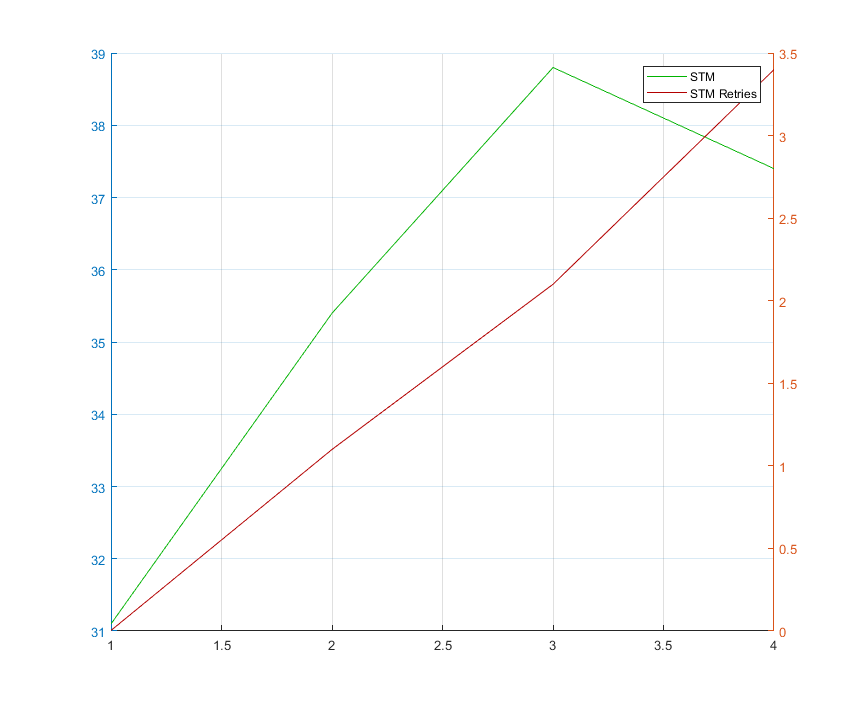
\includegraphics[width=0.6\textwidth, angle=0]{./fig/sugarscape/tvar_syncenv_500_50x50.png}
	\caption{Steps per second and retries on 50x50 grid and 500 initial agents using a \textit{TArray} on an asynchronous and synchronous environment.}
	\label{fig:tarray_results_syncenv_time}
\end{figure}

Now we are arriving at substantial performance improvements, which is directly reflected in the retry-ratios which are close to 0. Also this makes the point of this section crystal clear: selecting the right transactional data-structure is paramount for best performance when using STM. Out of interest we ran the \textit{TArray} implementation with a concurrent environment to see how much impact this has, and indeed it has some impact and reduces performance by quite some factor but is still considerable faster than a \textit{TVar} synchronous environment approach. What is interesting is that the performance on 2 cores drops below the one of 1 core TODO: why?.

TODO: figure which combines all the previous figures into one: TVar sync and async with TArray sync and async

\subsection{Scaling up Agents}
So far we always kept the initial number of agents at 500, which due to the model specification the number drops quickly to around 200 and stabilises around there due to the carrying capacity of the environment as described in the books \cite{epstein_growing_1996} section \textit{Carrying Capacity} (p. 30). We now want to see the scaling property of our approaches when increasing the number of agents. For this we slightly change the implementation: always when an agent dies it spawns a new one. This ensures that we keep the number of agents always constant (still fluctuates slightly between 500 and 490) over the whole duration. This ensures a constant load of concurrent processes interacting with each other and demonstrates also the ability to terminate and fork threads dynamically during the simulation.
Except for the Sequential approach we run all experiments with 4 cores with a concurrent environment. We look into the performance of 500, 1,000, 1,500, 2,000 and 2,500 (maximum possible capacity of the 50x50 environment). We also measured the average retries both for \textit{TVar} and \textit{TArray} under 2,500 agents  the \textit{TArray} approach shows best scaling performance with 0.01 retries whereas \textit{TVar} averages at 3.28 retries. Again this is can be attributed to the better transactional data-structure which reduces retry-ratio substantially to near-zero levels. The results are reported in Table \ref{tab:state_results_agentsscale_time} and can be seen in Figure \ref{fig:state_results_agentsscale_time}.

\begin{table}
	\centering
  	\begin{tabular}{ c || c | c | c }
        Agents  & Sequential & TVar       & TArray        \\ \hline \hline 
    	500     & 14.1       & 21.1       & \textbf{74.4} \\ \hline
   		1,000   & 6.8        & 11.3       & \textbf{56.8} \\ \hline
   		1,500   & 4.5        & 8.1        & \textbf{45.2} \\ \hline
   		2,000   & 3.3        & 6.2        & \textbf{37.0} \\ \hline 
   		2,500   & 2.6        & 5.2        & \textbf{31.7}
   	\end{tabular}
  	
  	\caption{Steps per second on 50x50 grid and varying number of agents.}
	\label{tab:state_results_agentsscale_time}
\end{table}

\begin{figure}
	\centering
	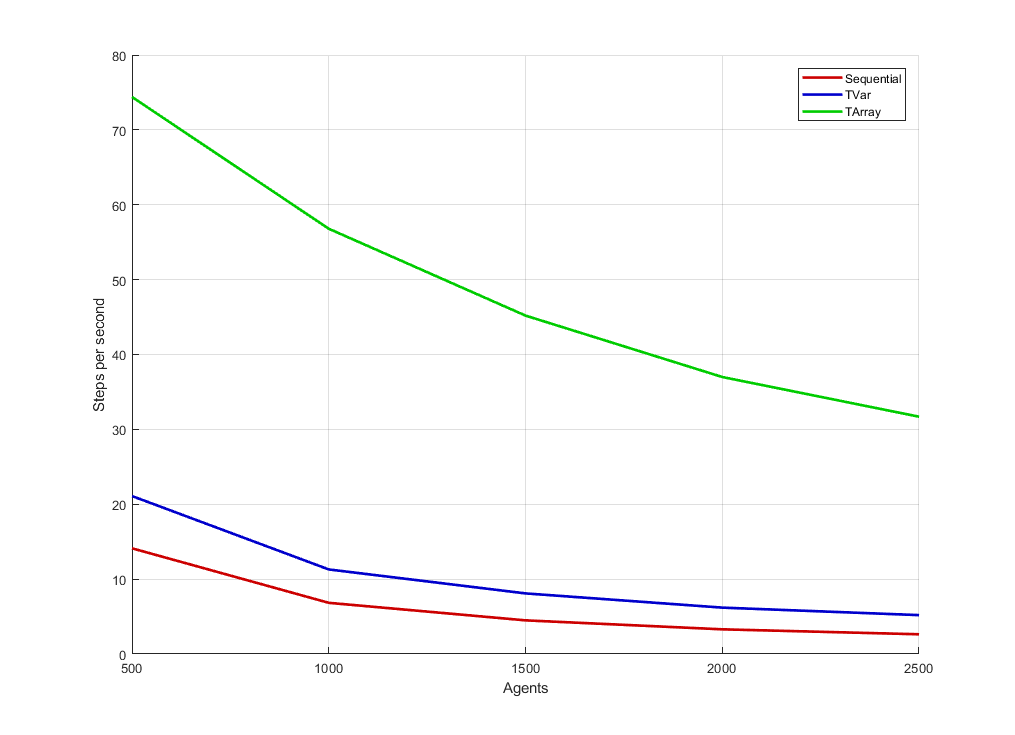
\includegraphics[width=0.6\textwidth, angle=0]{./fig/sugarscape/agents_performance.png}
	\caption{Steps per second on 50x50 grid and varying number of agents.}
	\label{fig:state_results_agentsscale_time}
\end{figure}

\subsection{Comparison with other approaches}
The paper \cite{lysenko_framework_2008} reports a performance of 17 steps in RePast (non-parallel), 18 steps in MASON and 2000 steps per seconds on a GPU on a 128x128 grid. Although our \textit{Sequential} implementation which runs non-parallel as well outperforms the RePast and MASON implementations one must be very well aware that these results were generated in 2008, on 10 year older hardware - the performance might have caught up by now and even outperform our functional sequential approach. 

Indeed, when we run the SugarScape example of RePast with the same model parameters as ours on the same machine (see Table \ref{tab:machine_specs}) we arrive at roughly 450 steps per second - a factor of more than 5 faster than even our STM implementation on 4 cores. This might seem quite shocking, even more so because RePast also performs visual output, rendering the SugarScape in every step. When scaling up the agents to 2,500 the RePast version arrives around roughly 95 steps per second which is still faster by a factor of 3 than our 4 core TArray implementation. Still our research is a first step and might result in future work increasing performance.

The very high performance on the GPU does not concern us here as it follows a very different approach than we do here. Our focus is on speeding up implementations on the CPU as directly as possible without locking overhead. When following a GPU approach one needs to map the model to the GPU which is a delicate and non-trivial approach. With our approach we show that speed-up with concurrency is very possible without the low-level locking details or the need to map to GPU.

Note that we kept the grid-size constant because we implemented the environment as a single agent which works sequentially on the cells to regrow the sugar. Obviously this doesn't really scale up on parallel hardware and indeed, the performance goes down dramatically when we increase the environment to 128x128 with same number of agents. Obviously this is the result of Amdahls law where the environment becomes the limiting factor of the simulation. Depending on the underlying data-structure used for the environment we have two options to solving this problem. In the case of the Sequential and TVar implementation we build on an indexed array which we can updated in parallel using the existing data-parallel support in Haskell (TODO: explain). In the case of the TArray approach we have no option but to run the update of every cell within its own thread. We leave both for further research as it is out of scope of this paper. 

\subsection{Discussion}
Interpretation of the performance data leads to the following insights:
